% Heat, Rain & Harvest - IEEE conference-style draft.
% Compile from reports/paper/:  pdflatex paper && bibtex paper && pdflatex paper && pdflatex paper
% Figures are read from ../figures/ (produced by the notebooks).
% BEFORE SUBMISSION: verify every reference entry against the original publication.
\documentclass[conference]{IEEEtran}
\usepackage{graphicx,booktabs,amsmath,siunitx,url}
\graphicspath{{../figures/}}

\begin{document}
\title{Heat, Rain and Harvest: District-Level Evidence on Climate Shocks, Irrigation and Wheat and Rice Yields in India, 1997--2022}

\author{\IEEEauthorblockN{Mehtaab and Pravansh}
\IEEEauthorblockA{MCA, Thapar Institute of Engineering and Technology, Patiala, India}}

\maketitle

\begin{abstract}
We build a district-level panel of wheat and rice yields for India (1997--2022) from official Directorate of Economics
and Statistics (DES) crop statistics, harmonised to fixed Census 2011 districts, and link it to India Meteorological
Department (IMD) gridded daily weather and DES land-use irrigation statistics. Using district and year fixed effects
with district-clustered errors, a \SI{1}{\degreeCelsius} warmer wheat-season night temperature is associated with a
4.6--5.8\% lower wheat yield across eight robustness variants. Irrigation clearly buffers monsoon rice against rainfall
deficits (interaction $p<0.0001$), whereas evidence that irrigation protects wheat against March heat is only suggestive
($p=0.10$). Despite these statistically robust effects, weather explains only about 1--2\% of out-of-sample yield
variation: on held-out years 2018--2022 the best model improves on a trend-only baseline by 1.8\% (wheat) and no model
improves for rice, and a pre-harvest forecast missed the 2022 heatwave losses in Punjab and Haryana. Under uniform
warming without adaptation, a fixed-effects model implies wheat yield changes of $-5.7\%$ [$-6.6$, $-4.8$] at
\SI{+1}{\degreeCelsius} and $-11.3\%$ [$-13.2$, $-9.4$] at \SI{+2}{\degreeCelsius}. We release the pipeline and an
interactive Crop-Climate Risk Atlas.
\end{abstract}

\begin{IEEEkeywords}
climate change, crop yield, panel data, fixed effects, India, wheat, rice, irrigation, heat stress
\end{IEEEkeywords}

\section{Introduction}
Wheat and rice are India's main staple crops, and both are exposed to rising temperatures and variable monsoon
rainfall. Field and satellite studies show that extreme heat accelerates wheat senescence in India \cite{lobell2012},
and panel studies elsewhere find strongly non-linear temperature effects on yields \cite{schlenker2009}; global
syntheses report yield losses with warming for both crops \cite{asseng2015,zhao2017}. District-level evidence for India
that (i) uses only official sources, (ii) handles India's frequent district boundary changes, and (iii) separates
explanation from out-of-sample prediction remains limited.

We ask three questions: (Q1) how strongly do heat and rainfall shocks move district wheat and rice yields?
(Q2) does irrigation weaken these effects? (Q3) can weather available before harvest forecast yields better than a
simple trend? Our contributions are a reproducible, official-source district panel on fixed Census 2011 units with a
validated mapping of post-2011 districts, a careful separation of significance from predictive skill, and an open
interactive atlas.

\section{Data}
\textbf{Crops.} DES Area--Production--Yield statistics (all 38 states/UTs, 1997--98 to 2022--23) give
406{,}612 district-season-crop-year records; after harmonisation, 388{,}399 records on 626 units. We analyse wheat
(12{,}323 district-years) and monsoon-season rice (kharif, autumn and winter rice; 14{,}379 district-years).

\textbf{Irrigation.} DES Land Use Statistics (1998--99 to 2022--23; 19{,}875 district-years) give crop-wise
irrigated area; irrigation share = irrigated area / crop area.

\textbf{Weather.} IMD gridded daily rainfall at \ang{0.25} \cite{pai2014} and maximum/minimum temperature at
\ang{1.0} \cite{srivastava2009}, 1997--2023, aggregated to districts by area-weighted averaging of grid-cell/district
intersections in an equal-area projection.

\textbf{Boundaries.} Census 2011 district polygons from the SHRUG Open Polygons (Development Data Lab, version 2.2;
also hosted on the Government of India AIKosh portal) \cite{asher2021}; 640 districts.

\section{Methods}
\subsection{Harmonisation to fixed districts}
Current district names were matched to the Local Government Directory (LGD) by exact normalised name within the
state and its successor states (e.g.\ Jharkhand from Bihar), plus 80 reviewed renames. LGD gives each district's
Census 2011 code. For the 152 districts created after 2011, the parent was derived from sub-districts: each current
tehsil's Census 2011 sub-district code was mapped to its 2011 district. Applied to districts that existed in 2011,
this rule reproduced the known code for 625 of 627 (99.7\%). Twenty-seven new districts drew tehsils from several
parents and were assigned to the majority parent; Tripura's 2012 districts could not be traced and Tripura is treated
as one unit. Area and production were summed and yield recomputed as production/area.

\subsection{Data quality}
Physically implausible yields (above \SI{7}{t/ha} for wheat or \SI{8}{t/ha} for rice, or more than three times away
from the district's own median) were flagged and excluded (0.8\% of wheat and 1.8\% of rice district-years). We found
a break in Madhya Pradesh's reported wheat area and production from 2018 (area roughly doubling while yields stayed in
range); national averages use fixed area weights, all models include year effects, and results are re-estimated
without Madhya Pradesh 2018+.

\subsection{Features}
Wheat season: 1 Nov to 31 Mar (so all wheat predictions are pre-harvest); rice: 1 Jun to 31 Oct. Features: mean
maximum and minimum temperature, growing degree days, extreme degree days above \SI{34}{\degreeCelsius} (wheat) or
\SI{35}{\degreeCelsius} (rice), days above \SI{35}{\degreeCelsius} in March, seasonal and monthly rainfall, rainy days,
rainfall variability and the longest monsoon dry spell. Yields are expressed as relative deviations from a
district-specific linear trend.

\subsection{Inference}
Our main specification is
\begin{equation}
y_{dt} = \beta\,W_{dt} + \gamma\,(W_{dt}\times I_{dt}) + \delta\,I_{dt} + \alpha_d + \tau_t + \varepsilon_{dt},
\end{equation}
where $y_{dt}$ is the relative yield anomaly of district $d$ in year $t$, $W$ weather, $I$ irrigation share, $\alpha_d$
and $\tau_t$ district and year fixed effects; standard errors are clustered by district. Classical tests (t, z, ANOVA,
chi-square, multiple-testing corrections, cluster bootstrap) are reported in the supplementary notebook.

\subsection{Prediction}
Train 1997--2017, test 2018--2022. Trends, district means, scaling and tuning (GroupKFold over years) use training
years only; same-year irrigation is replaced by each district's training-period mean because it is not known before
harvest. Baseline: extrapolated district trend. Models: within-district OLS, Ridge, random forest, gradient boosting,
and yield-loss classifiers (loss = more than 10\% below trend). Skill $=1-\mathrm{MSE}/\mathrm{MSE}_{\text{baseline}}$.
After a weak first run we tried agronomy-motivated features (February heat, heat above \SI{30}{\degreeCelsius},
preceding-monsoon rain, rain as a share of normal, monsoon-only rice) and chose between versions by cross-validation on
training years only.

\subsection{Warming scenarios}
We add \SI{1}{\degreeCelsius} or \SI{2}{\degreeCelsius} to every daily maximum and minimum temperature, recompute
all features, and apply the fixed-effects model to the 2018--22 seasons. Uncertainty: cluster bootstrap over districts
(300 resamples, model refitted each time).

\section{Results}
\subsection{Heat, rain and irrigation}
A warmer wheat-season night is the most consistent signal: $-5.3\%$ per \SI{1}{\degreeCelsius} [95\% CI $-6.6$,
$-4.0$] in the main sample and $-4.6\%$ to $-5.8\%$ across eight variants (Fig.~\ref{fig:robust}). Ten more days
above \SI{35}{\degreeCelsius} in March lower wheat yield by 1.8\% at average irrigation ($p=0.017$). In the 2022
heatwave season Punjab and Haryana yields were 9.5\% below trend [$-11.6$, $-7.4$], while most of central India was
near trend despite comparable extra heat. For monsoon rice, a 20\% rainfall deficit reduces yield by about 3.1\% at
20\% irrigation but only 0.3\% at 95\% irrigation (interaction $p<0.0001$). For wheat, the heat$\times$irrigation
interaction points in the protective direction but is not significant ($p=0.10$; $p=0.045$ without Madhya Pradesh
2018+).

\begin{figure}[t]
\centering
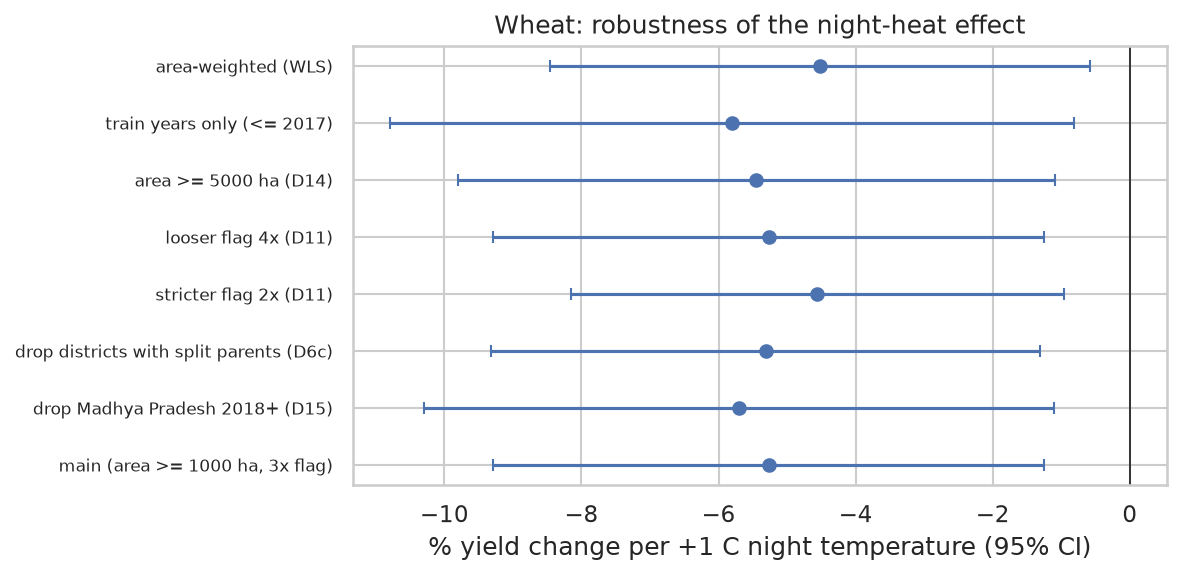
\includegraphics[width=\columnwidth]{08_robustness_wheat.png}
\caption{Effect of +\SI{1}{\degreeCelsius} wheat-season night temperature on yield across sample variants (district
and year fixed effects, clustered 95\% CI).}
\label{fig:robust}
\end{figure}

\subsection{Risk zones}
K-means on district profiles (silhouette-optimal $k=5$; agreement with Ward clustering ARI $=0.61$) yields
geographically coherent zones although no coordinates were used, from the irrigated north-west (15\% loss years) to
Madhya Pradesh and Bihar (34\% loss years, highest heat sensitivity despite 83\% irrigation). Graph-based label
propagation recovered hidden risk labels with balanced accuracy 0.64 (supervised kNN 0.59; chance 0.50).

\subsection{Prediction}
\begin{table}[t]
\caption{Out-of-sample skill vs the trend-only baseline, test years 2018--2022}
\label{tab:skill}
\centering
\begin{tabular}{lrr}
\toprule
Model & Wheat & Rice (monsoon) \\
\midrule
Within-district OLS & $-4.0\%$ & $-2.9\%$ \\
Ridge & $+1.8\%$ & $-2.4\%$ \\
Random forest & $+0.7\%$ & $-3.1\%$ \\
Gradient boosting & $-3.9\%$ & $-3.9\%$ \\
\bottomrule
\end{tabular}
\end{table}
Table~\ref{tab:skill} shows that no model materially beats the trend: random forest was 21\% better than the baseline
in-sample but under 1\% out of sample. Loss classifiers (wheat ROC-AUC 0.56--0.58) did not beat each district's
historical loss frequency (0.58). The pre-harvest forecast for 2021--22 predicted $+3.7\%$ for Punjab--Haryana against
an observed $-12.3\%$ relative to the training trend.

\subsection{Warming scenarios}
Without adaptation, modelled wheat yield changes are $-5.7\%$ [$-6.6$, $-4.8$] at \SI{+1}{\degreeCelsius} and
$-11.3\%$ [$-13.2$, $-9.4$] at \SI{+2}{\degreeCelsius}; for monsoon rice $-4.4\%$ [$-5.7$, $-2.6$] and $-7.5\%$
[$-10.4$, $-3.7$]. These are consistent in sign and broadly in magnitude with global syntheses \cite{asseng2015,zhao2017}.
Less-irrigated districts show larger modelled losses (wheat at \SI{+2}{\degreeCelsius}: $-29\%$ below 50\% irrigation
vs $-9\%$ above 90\%), but these are mostly hill districts, so irrigation and location are confounded.

\section{Discussion}
Heat effects are real and robust, yet small relative to all other sources of year-to-year variation (yield anomalies
have a standard deviation of about 19\%), so statistical significance does not translate into forecast skill.
Districts' historical risk is about as informative as this year's weather for predicting loss years. Irrigation
clearly protects rice against monsoon deficits; for wheat, water cannot fully offset heat during grain filling, which
is consistent with the high heat sensitivity of the irrigated Madhya Pradesh--Bihar zone.

\section{Limitations}
\begin{itemize}
\item \textbf{Weather resolution:} temperature is on a \ang{1} grid (about \SI{110}{km}); 64 districts lie within a single cell and neighbouring districts share temperature series.
\item \textbf{Boundaries:} the PC11 polygons are compiled from several sources (SEDAC, Bharatmaps, Datameet, Administrative Atlas of India) with up to about \SI{1}{km} error; 27 split districts are assigned to a majority parent; Tripura is one unit.
\item \textbf{Data quality:} a reporting break in Madhya Pradesh wheat area/production from 2018; implausible yields flagged by rule (threshold sensitivity checked); LUS and APY irrigation and crop areas are collected separately (irrigation share sometimes above 1); irrigation starts in 1998--99; LUS irrigated rice covers all seasons.
\item \textbf{Seasons:} fixed calendar windows ignore district-specific sowing dates.
\item \textbf{Identification:} fixed effects remove stable district differences and common year shocks, but time-varying confounders (e.g.\ input use, pests) remain; irrigation is not randomly assigned.
\item \textbf{Prediction:} test period is five years; trend extrapolation error dominates; a few test-set comparisons were made before features were selected by training-year CV (disclosed).
\item \textbf{Scenarios:} uniform warming, unchanged rainfall, no adaptation, linear model; \SI{+2}{\degreeCelsius} extrapolates beyond observed variation.
\end{itemize}

\section{Conclusion}
Using only official data harmonised to fixed districts, we find robust negative effects of warmer nights on Indian
wheat yields and strong irrigation buffering of rice against monsoon deficits, but very limited out-of-sample
predictability of yields from weather alone. Policy-relevant risk maps should therefore combine historical risk with
climate sensitivity rather than rely on seasonal weather forecasts alone.

\section*{Data and code availability}
All code, decisions and the Crop-Climate Risk Atlas are in the project repository; raw data are downloadable from the
cited official portals.

\bibliographystyle{IEEEtran}
\bibliography{references}
\end{document}
